\documentclass[page number]{beamer}
\usetheme[sectionpage=none,numbering=fraction,progressbar=foot]{metropolis}

\usepackage{pgf,tikz}
\usetikzlibrary{arrows}
\usetikzlibrary{positioning,shapes,fit}
\usepackage{xcolor}
\usepackage{amssymb}
\usepackage{amsmath}

\makeatletter
\makeatother

\setcounter{tocdepth}{1} % remove subsection from table of contents

% colors
\definecolor{mDarkRed}{HTML}{6F1616}
\definecolor{mDarkGreen}{HTML}{106235}
\definecolor{mTeal}{HTML}{112233}
\definecolor{mBlack}{HTML}{000000}
\setbeamercolor{normal text}{fg=mTeal}
\setbeamercolor{alerted text}{fg=mDarkRed}
\setbeamercolor{example text}{fg=mDarkGreen}
\setbeamercolor{title separator}{fg=purple,bg=mBlack}

\definecolor{spec}{HTML}{6F1616}
\definecolor{prog}{HTML}{106235}

\def\outline{
  \begin{frame}[plain,noframenumbering]
    \frametitle{Outline}
    \tableofcontents[currentsection]
  \end{frame}
}


\begin{document}
\title[QCHL]{Precise Detection of Side-Channel Vulnerabilities using Quantitative Cartesian Hoare Logic}

\author[Aur\`ele Barri\`ere]{Aur\`ele Barri\`ere}

\date{\textit{ENS Rennes}
  \vfill
  \textbf{April 16, 2018}}

\def\outline{
  \begin{frame}[plain,noframenumbering]
    \frametitle{Outline}
    \tableofcontents[currentsection]
  \end{frame}
}

\begin{frame}[plain,noframenumbering]
  \vspace{-2cm}
  \maketitle
  \vspace{-4cm}
\end{frame}

%% \metroset{sectionpage=none}

%% \metroset{sectionpage=progressbar}

\def\spec#1{{\color{spec}\textbf{#1}}}
\def\prog#1{{\color{prog}\textbf{#1}}}

\section{Cartesian Hoare Logic}
\begin{frame}{Cartesian Hoare Logic for Verifying $k$-Safety Properties}
  \begin{center}
    Marcelo Sousa\qquad Isil Dillig\\
    PLDI 2016
  \end{center}
  \vfill
  \begin{exampleblock}{Contribution}
    \begin{itemize}
    \item Cartesian Hoare Logic: \textbf{sound} and \textbf{complete}
    \item Automated tool for verification: \textsc{Descartes}
    \item Verification of realistic examples. \textbf{bugs found}
    \end{itemize}
  \end{exampleblock}
\end{frame}

\begin{frame}{Reminder: Hoare Logic}
  \begin{block}{Hoare Logic}
    \begin{itemize}
    \item \spec{Specification} language
    \item \prog{Program} language
    \item Logic rules to prove \textbf{Hoare Triples}
    \end{itemize}
  \end{block}
  \vfill
  \begin{block}{Hoare Triple}
    $$\{ \spec{$\phi$} \}\quad \prog{S} \quad\{ \spec{$\psi$} \}$$
    \begin{center}
      Precondition\quad Program\quad Postcondition
    \end{center}
  \end{block}
  \vfill
  \begin{exampleblock}{Hoare Triple's meaning}
    Any terminating execution of \prog{S} from a state where \spec{$\phi$} holds
    ends on a state where \spec{$\psi$} holds.
  \end{exampleblock}
\end{frame}

\begin{frame}{Hoare Logic's rules}
  \begin{center}
    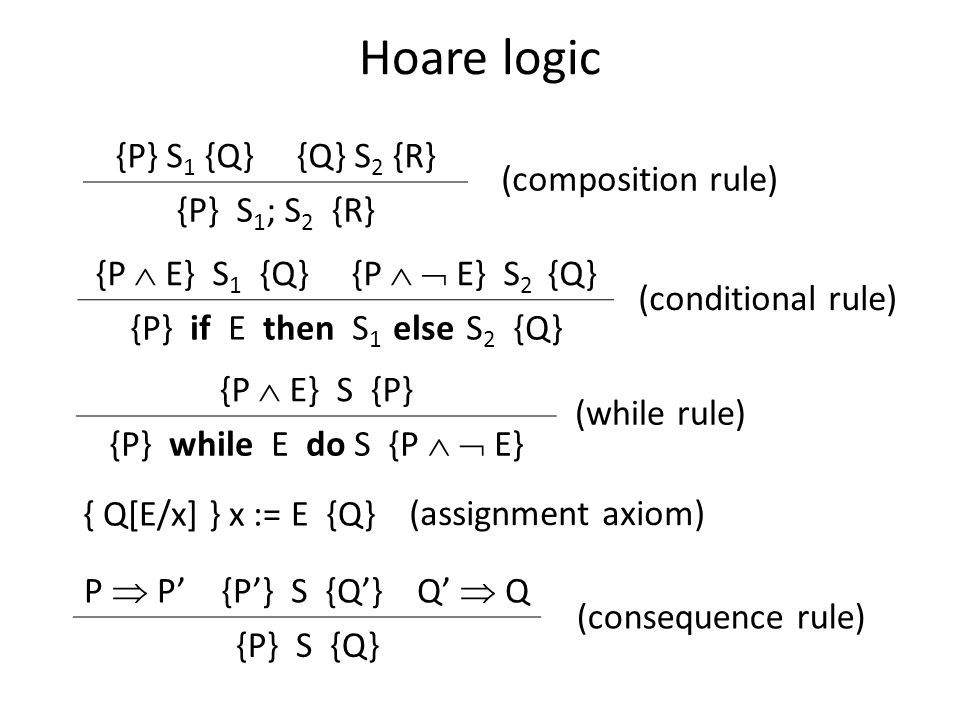
\includegraphics[scale=0.4]{img_sousa/hoare.jpg}
  \end{center}
\end{frame}
\begin{frame}{Hoare Logic Properties}

  \begin{exampleblock}{Properties}
    \begin{itemize}
    \item Expressive
    \item Not decidable
    \item Well-studied
    \item Many extensions
    \end{itemize}
  \end{exampleblock}

\end{frame}

\begin{frame}{$k$-Safety Properties}
  \begin{alertblock}{Motivation}
    Some correctness properties require reasonning about multiple program executions and their relationship.\\
    These are \textbf{$k$-Safety Properties} ($k$ : nb of executions).\\
    Introduced by Clarkson and Schneider in \textbf{Hyperproperties} (CSF2008).\\
    Hoare Logic only reasons about \textit{any single} execution of a program.
  \end{alertblock}
  \vfill
  \begin{exampleblock}{Example: 2-safety hyperproperty}
    Determinism: $\forall \prog{S},x,y,\quad\prog{S}(x) = \prog{S}(y)$.
  \end{exampleblock}
\end{frame}

\def\comp{\prog{\texttt{compare}}}

\begin{frame}{Comparator Example}

  \comp\ Java methode.
  \begin{enumerate}
  \item $\forall x,y, sgn(\comp(x,y)) = -sgn(\comp(y,x))$
  \item $\forall x,y,z, (\comp(x,y)>0\wedge \comp(y,z)>0)\rightarrow \comp(x,z)>0$
  \item $\forall x,y,z, (\comp(x,y)=0\rightarrow (sgn(\comp(x,z))=sgn(\comp(y,z))))$
  \end{enumerate}
\end{frame}

\begin{frame}{Buggy Comparator}
  \begin{center}
    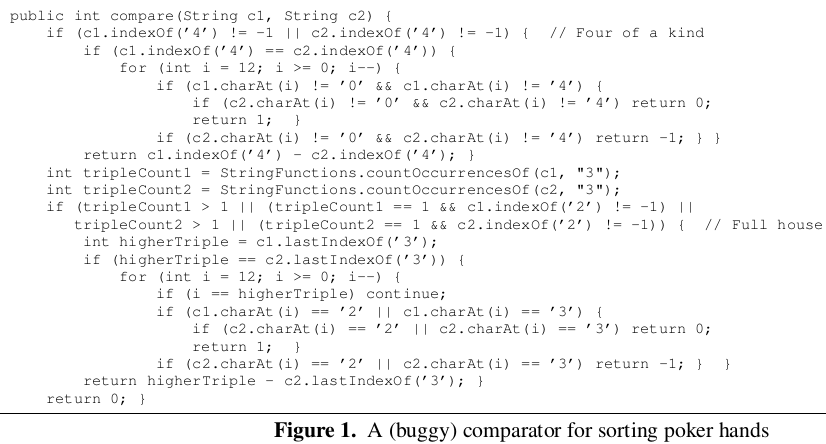
\includegraphics[scale=0.4]{img_sousa/buggycomp.png}
  \end{center}
\end{frame}

\begin{frame}{Cartesian Hoare Logic}

  \begin{block}{Cartesian Hoare Triple}
    $$||\spec{$\phi$}||\quad\prog{S}\quad||\spec{$\psi$}||$$
  \end{block}
  \vfill
  \begin{block}{Example}
    $$||\spec{$y_1=x_2\wedge x_1=x_3\wedge y_2=y_3$}||$$
    $$\quad\comp(x,y)$$
    $$||\spec{$ret_1 > 0\wedge ret_2>0 \rightarrow ret_3 >0$}||$$
  \end{block}
  \vfill
  \begin{block}{Meaning}
    Forall $(\pi_1,\dots,\pi_k)$, where $\pi_i$' inputs are $(x_i,y_i)$, $\pi_i$'s output is $ret_i$, and the set of inputs satisfy the precondition, the postcondition holds.
  \end{block}
  
\end{frame}

\begin{frame}{Program Language}
  \begin{center}
    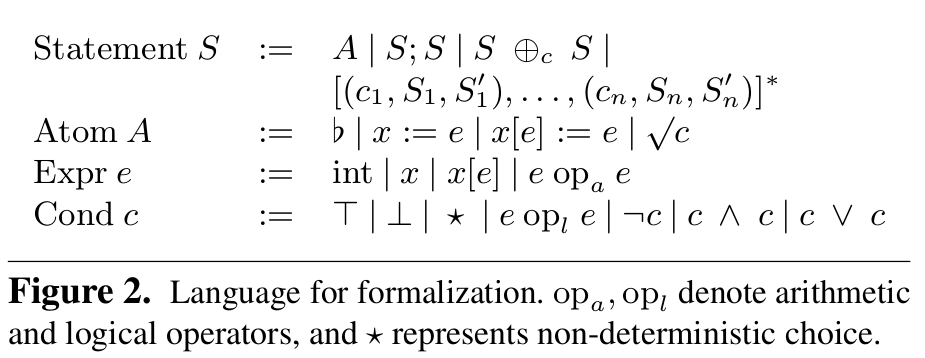
\includegraphics[scale=0.3]{img_sousa/proglang.png}
  \end{center}
\end{frame}

\begin{frame}{Semantics}
  
  \begin{block}{Operational semantics}
    $$\sigma,e\Downarrow \texttt{int}\quad\quad\sigma,\prog{S}\Downarrow \sigma'$$
  \end{block}
  \vfill
  \begin{block}{Entailment}
      $$\sigma\models\varphi\quad iff\quad \sigma,\varphi\Downarrow \texttt{true}$$
  \end{block}
  \vfill
  \begin{block}{Equivalence}
    $$\prog{S$_1$}\equiv\prog{S$_2$} \text{ if}\quad\forall \sigma,\sigma', \quad \sigma,\prog{S$_1$}\Downarrow\sigma'\ iff\  \sigma,\prog{S$_2$}\Downarrow\sigma'$$
  \end{block}
  \vfill
  \begin{block}{Valid Hoare Triple}
    $$\{ \spec{$\phi$} \}\ \prog{S}\ \{ \spec{$\psi$} \}\text{ valid } iff\ \forall(\sigma,\sigma')$$
    $$\text{if }\sigma\models\phi\text{ and } \sigma,\prog{S}\Downarrow\sigma'\text{ then }\sigma'\models\psi$$
  \end{block}
    
  
\end{frame}

\begin{frame}{Valid Cartesian Horae Logic Triple}
  \begin{block}{Validity}
  \begin{center}
    $||\spec{$\phi$}||\quad\prog{S}\quad||\spec{$\psi$}||$ valid $\ iff\ $\\
    $\forall \{(\sigma_1,\sigma_1'),\dots,(\sigma_k,\sigma_k')\}$ such that
    $\biguplus_{i}\ \sigma_i\models\spec{$\phi$}$ and $\forall i, \sigma_i,\prog{S}\Downarrow\sigma_i'$,\\
     we also have $\biguplus_{i}\ \sigma_i'\models\spec{$\psi$}$

  \end{center}
  \end{block}
  \vfill
  \begin{block}{Counter-example}
    $k$ executions of \prog{S}.
  \end{block}
\end{frame}

\begin{frame}{Cartesian Hoare Triple Examples}
    \begin{center}
    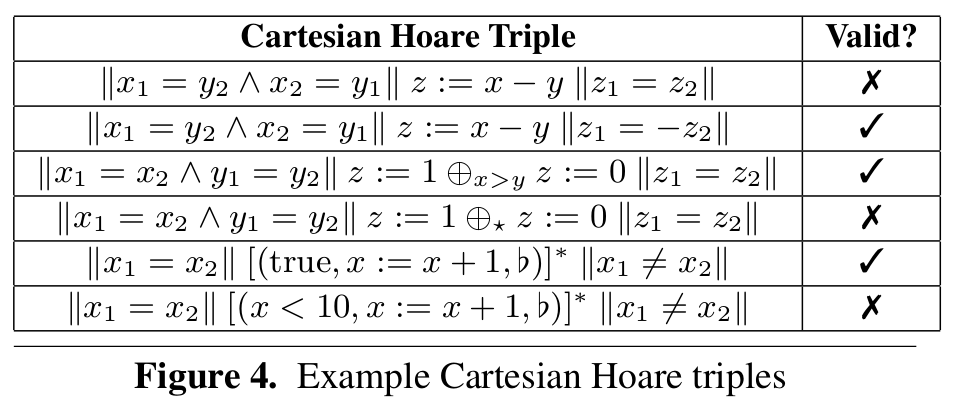
\includegraphics[scale=0.3]{img_sousa/fig4.png}
  \end{center}
\end{frame}

\begin{frame}{$k$-Safety properties Examples}
    \begin{center}
    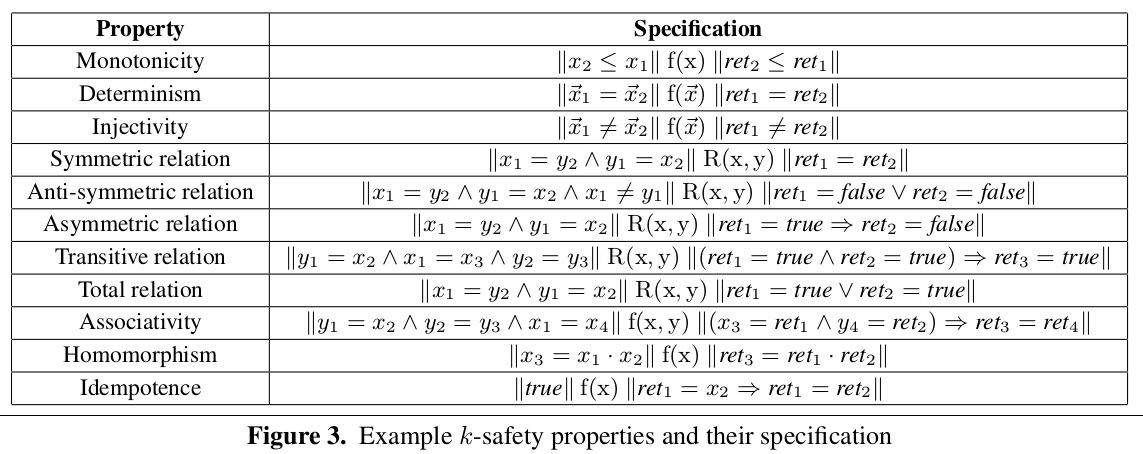
\includegraphics[scale=0.25]{img_sousa/fig3.png}
  \end{center}
\end{frame}

\begin{frame}{Program product}
  \begin{center}
    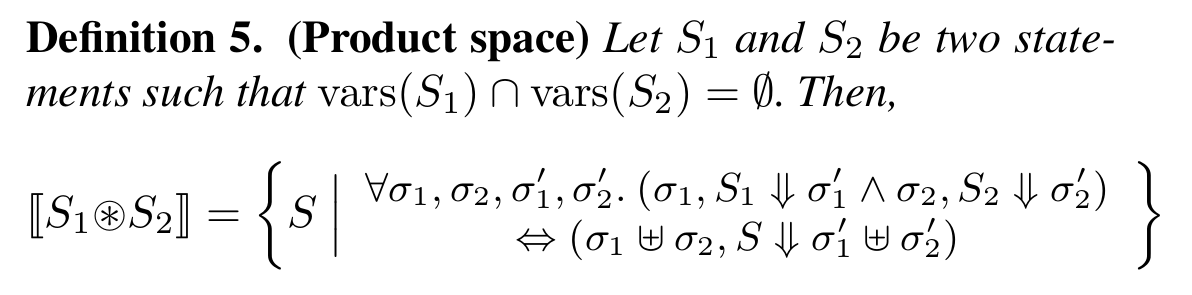
\includegraphics[scale=0.2]{img_sousa/def5.png}
  \end{center}
  \vfill
  \begin{exampleblock}{Meaning}
    The set of all programs semantically equivalent to the simultaneous execution of \prog{S$_1$} and \prog{S$_2$}
  \end{exampleblock}
  \vfill
  \begin{center}
    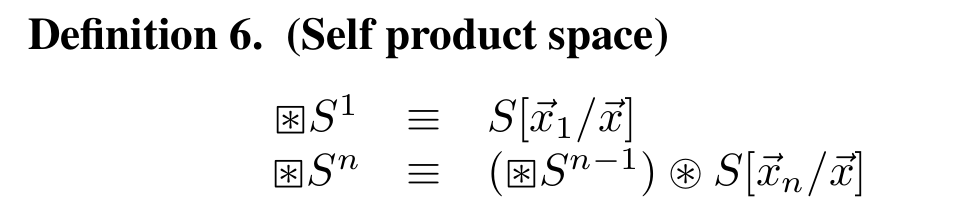
\includegraphics[scale=0.2]{img_sousa/def6.png}
  \end{center}
  
\end{frame}

\begin{frame}{Core Cartesian Hoare Logic Rules}
  \begin{center}
    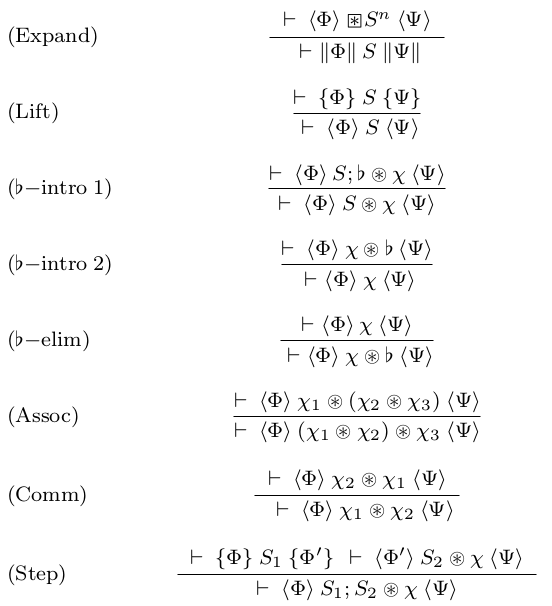
\includegraphics[scale=0.28]{img_sousa/rules1.png}
    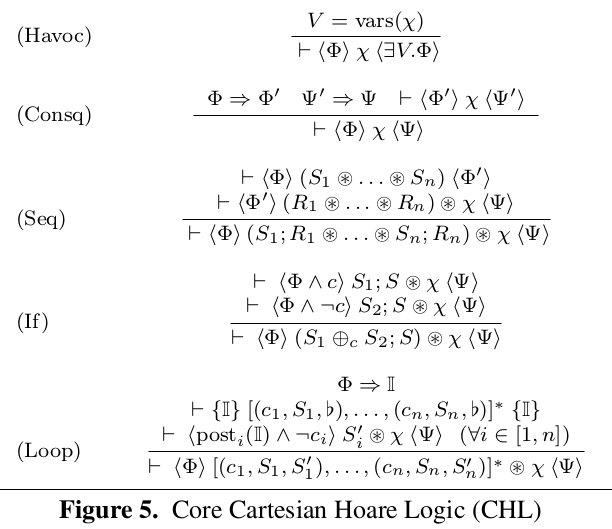
\includegraphics[scale=0.28]{img_sousa/rules2.png}
  \end{center}
\end{frame}

\begin{frame}{Cartesian Loop Logic}
    \begin{center}
    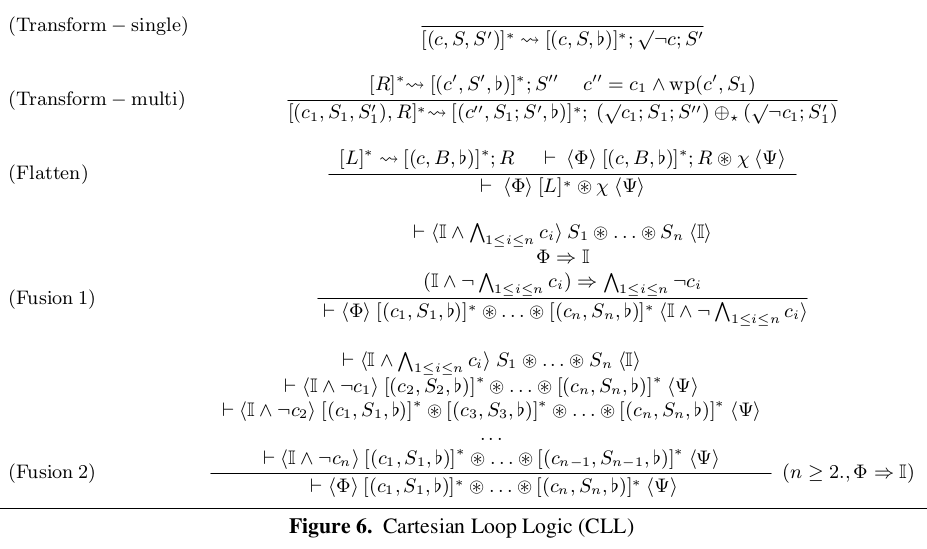
\includegraphics[scale=0.36]{img_sousa/fig6.png}
  \end{center}
\end{frame}

\begin{frame}{Theorems}
  \begin{exampleblock}{Soundness}
    If $\vdash ||\spec{$\phi$}||\ \prog{S}\ ||\spec{$\psi$}||$ then $\models ||\spec{$\phi$}||\ \prog{S}\ ||\spec{$\psi$}||$
  \end{exampleblock}
  \vfill
  \begin{exampleblock}{Relative Completeness}
    If we can decide the validity of a standard Hoare Triple, then\\
    if $\models ||\spec{$\phi$}||\ \prog{S}\ ||\spec{$\psi$}||$ then $\vdash ||\spec{$\phi$}||\ \prog{S}\ ||\spec{$\psi$}||$
  \end{exampleblock}
\end{frame}

\begin{frame}{Verification Algorithm}
  \begin{itemize}
  \item Use (Havoc), (Consq) and (If) as much as possible.
  \item Call to a Standard Hoare Logic prover.
  \item Step through matching loops using Cartesian Loop Logic.
  \item External procedure to find loop invariants.
  \end{itemize}
  \vfill
  \begin{exampleblock}{Theorem}
    The algorithm terminates for any Precondition, Postcondition and Program.
  \end{exampleblock}
  \vfill
  \begin{block}{Implementation}
    \textsc{Descartes} in Haskell. Uses Z3 for formula satisfiability.
  \end{block}
\end{frame}

\begin{frame}{Evaluation: StackOverflow}
    \begin{center}
    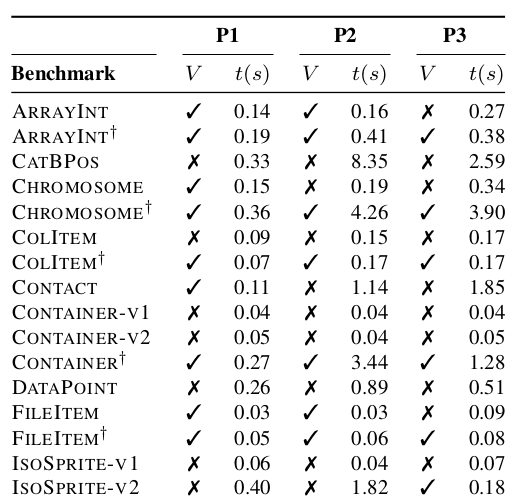
\includegraphics[scale=0.3]{img_sousa/91.png}
    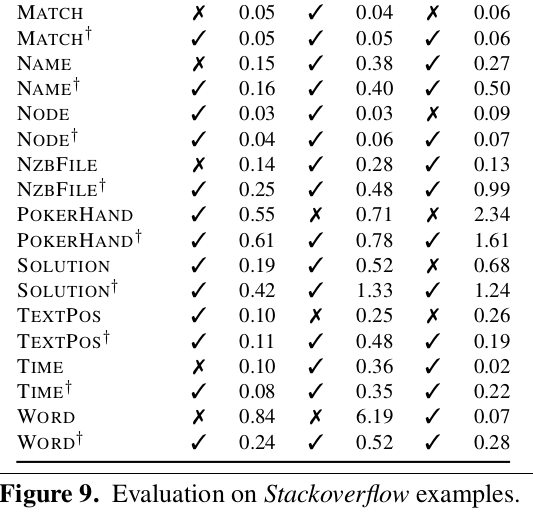
\includegraphics[scale=0.3]{img_sousa/92.png}
  \end{center}
\end{frame}

\begin{frame}{Evaluation: StackOverflow}
  \begin{itemize}
  \item No false alarms.
  \item Fast (1.21 seconds on average).
  \item Z3 gives a counter-example for invalid properties.
  \end{itemize}
\end{frame}

\begin{frame}{Evaluation: Github Projects}
  \begin{itemize}
  \item Apache Storm, ligGDX, Android, Netty. 2KLOC.
  \item  28 comparators. 34 equality methods.
  \item On average 9.14 seconds per method. (Maximum: 55.27sec)
  \item 5 false alarms.
  \item 5 real bugs discovered.
  \end{itemize}
\end{frame}

\begin{frame}{Related Works}
  \begin{block}{Self-Composition}
    Generates $k$ copies of the program sequentially. Verify a standard Hore Logic Triple. 20 times slower.
  \end{block}
  \vfill
  \begin{block}{Product Programs}
    No way to construct such product programs.
    Approximately 20 times slower.
  \end{block}
\end{frame}

\begin{frame}{Conclusion}
  \begin{itemize}
  \item New approach for automated verification of $k$-safety properties.
  \item Uses the similarity of program copies.
  \item Algorithm implemented. Bugs found.
  \end{itemize}
\end{frame}

\section{Quantitative Cartesian Hoare Logic}
\begin{frame}{Precise Detection of Side-Channel Vulnerabilities using Quantitative Cartesian Hoare Logic}
  \begin{center}
    Jia Chen\qquad Yu Feng \qquad Isil Dillig\\
    PLDI 2016
  \end{center}
  \vfill
  \begin{exampleblock}{Contribution}
    \begin{itemize}
    \item $\epsilon$-bounded non-interference.
    \item Quantitative Cartesian Hoare Logic.
    \item Implementation: \textsc{Themis}. Bugs found.
    \end{itemize}
  \end{exampleblock}
\end{frame}

\begin{frame}{Side channel attacks}
  \begin{itemize}
  \item Timing side channels
  \item Compression side channels
  \end{itemize}
  \vfill
  \begin{alertblock}{Vulnerabilities}
    Resource usage of the program (time, space, power, etc.) should not vary with respect to the secret.
  \end{alertblock}
  \vfill
  \begin{exampleblock}{$\epsilon$-bounded non interference}
    Resource usage does not vary by more than $\epsilon$.\\
    2-safety property.
  \end{exampleblock}
  
\end{frame}

\begin{frame}{Timing attack Example}
  \begin{center}
    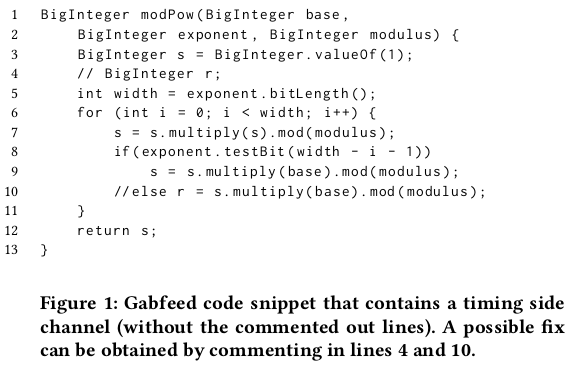
\includegraphics[scale=0.38]{img_chen/1.png}\\
    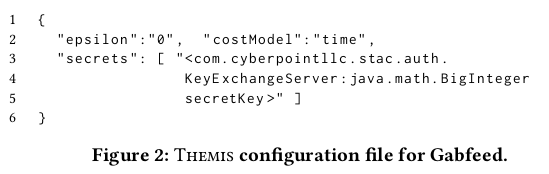
\includegraphics[scale=0.38]{img_chen/2.png}
  \end{center}
\end{frame}

\begin{frame}{Verification approach}
  \begin{enumerate}
  \item User specifies a value for $\epsilon$, type of attack and secret.
  \item \textsc{Themis} uses Taint Analysis to over-estimate the functions in which there can be a vulnerability.
  \item \textsc{Themis} uses Quantitative Cartesian Hoare Logic to find vulnerabilities.
  \item User changes the value of $\epsilon$. The usage difference can be proportional to the secret.
  \item User can try to repair the program. Run \textsc{Themis} on the repaired program
  \end{enumerate}
  \vfill
  \begin{alertblock}{Threat Model}
    Finds vulnerabilities only at the software level. Side channels at the microarchitecture level (cache contention, branch prediction) can't be found with this approach.
  \end{alertblock}
\end{frame}

\begin{frame}{Bounded non-interference}
  $P$ program. $\overrightarrow{a}$ input. $R_p(\overrightarrow{a})$ resource usage.
  \vfill
  \begin{block}{Non-interference}
    \begin{center}
      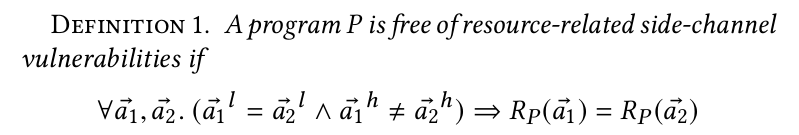
\includegraphics[scale=0.3]{img_chen/def1.png}
    \end{center}
  \end{block}
  \vfill
  \begin{block}{$\sigma$-bounded non-interference}
    \begin{center}
      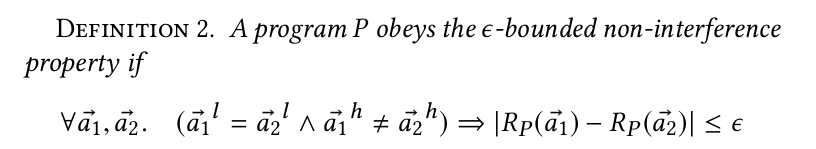
\includegraphics[scale=0.3]{img_chen/def2.png}
    \end{center}
  \end{block}    
\end{frame}

\begin{frame}{Quantitative Cartesian Hoare Logic - Program Language}
  \begin{center}
    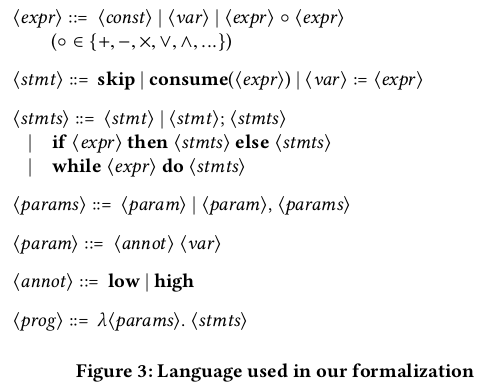
\includegraphics[scale=0.25]{img_chen/3.png}\\
    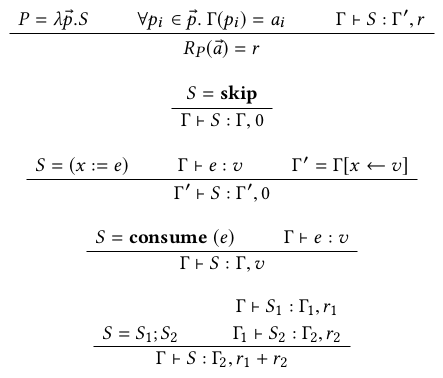
\includegraphics[scale=0.3]{img_chen/41.png}
    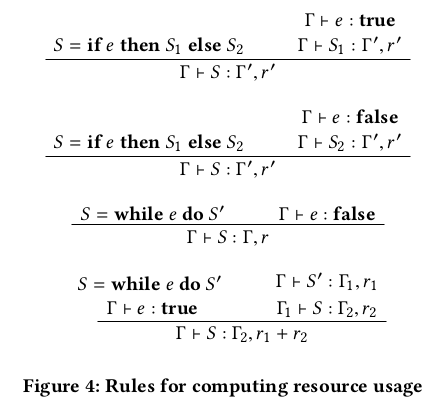
\includegraphics[scale=0.3]{img_chen/42.png}
  \end{center}
\end{frame}

\begin{frame}{Quantitative Cartesian Hoare Logic - Deterministic Proof rules}
  $\Sigma$: Taint environment.
\begin{center}
    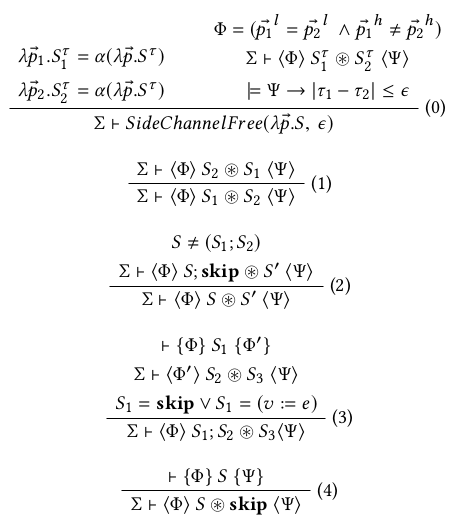
\includegraphics[scale=0.3]{img_chen/51.png}
    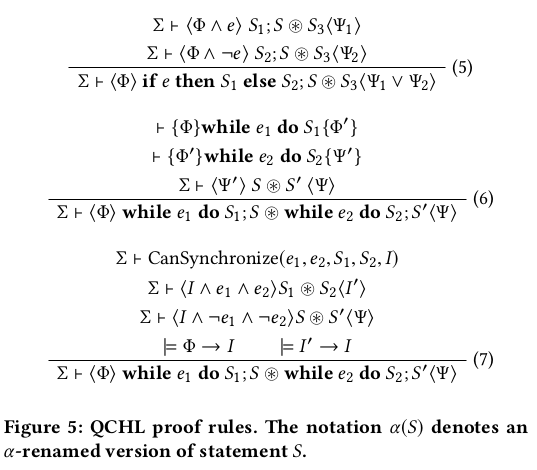
\includegraphics[scale=0.3]{img_chen/52.png}
\end{center}
\end{frame}

\begin{frame}{Synchronizing loops}
  $I$: relational loop invariant.
  \vfill
  \begin{center}
    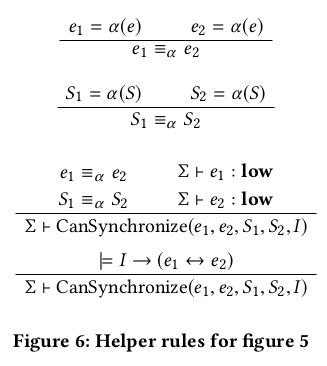
\includegraphics[scale=0.4]{img_chen/6.png}
  \end{center}
\end{frame}

\begin{frame}{Finding Relational Loop Invariants: Guess and Check}
  \begin{center}
    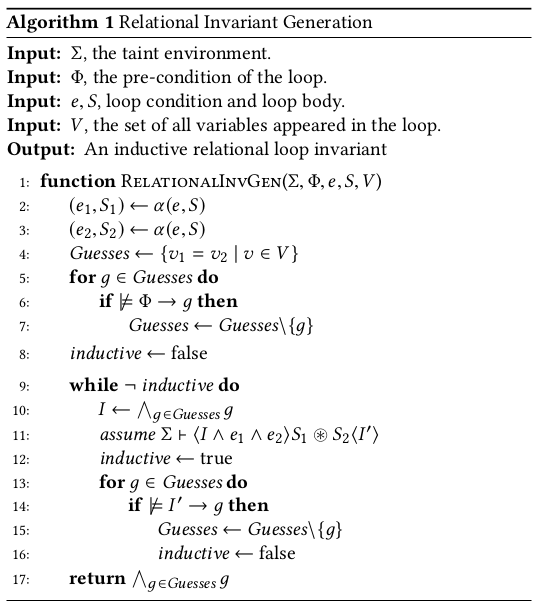
\includegraphics[scale=0.35]{img_chen/algo1.png}
  \end{center}
\end{frame}

\begin{frame}{Implementation}
  \begin{center}
    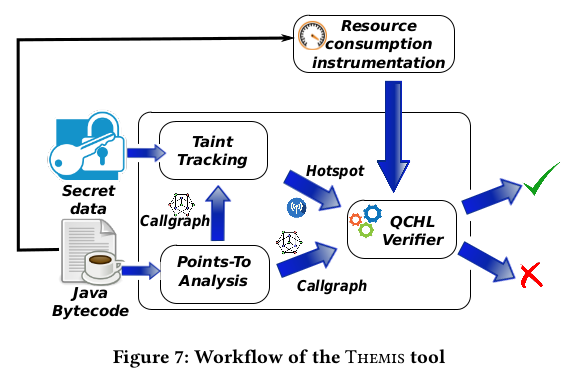
\includegraphics[scale=0.35]{img_chen/7.png}
  \end{center}
  \textbf{Pointer Analysis:} Creates callgrap, identify all variables that may alias.\\
  \textbf{Taint Analysis:} Find hotspots, synchronized loops.\\
  \textbf{Resource consumption instrumentation:} Adds the \texttt{consume} statements.
\end{frame}

\begin{frame}{False Alarm Example}
  \begin{center}
    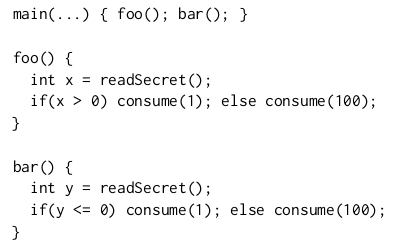
\includegraphics[scale=0.4]{img_chen/foobar.png}
  \end{center}
  \vfill
  No Side-Channel Vulnerbility here, but both functions will be seen as unsafe hotspots.
\end{frame}

\begin{frame}{Dependencies}
  \begin{itemize}
  \item \textbf{Z3:} SMT solver. Finds counterexamples.
  \item \textbf{FlowDroid:} Taint analyzer.
  \item \textbf{Apron:} numerical abstract domain library. Infer standard loop invariants.
  \item \textbf{Soot:} Framework for Java analysis. Transforms program syntax.
  \end{itemize}
\end{frame}

\begin{frame}{Evaluation: Comparison Against \textsc{Blazer}}
  \begin{block}{\textsc{Blazer}}
    Static analyzer for timing attacks. Standard non-interference.
  \end{block}
  \vfill
\begin{center}
    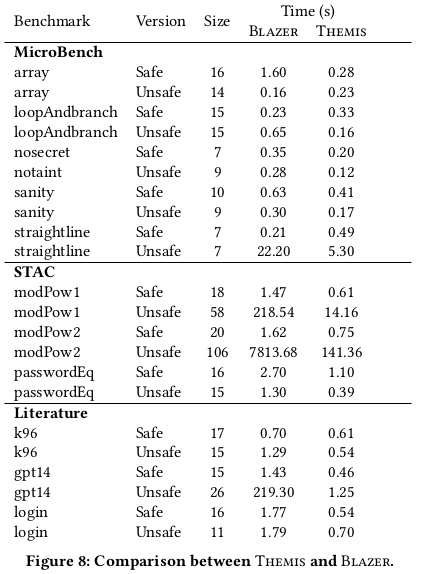
\includegraphics[scale=0.28]{img_chen/8.png}
  \end{center}
  \vfill
  \textsc{Themis} median: 7.73 seconds. \textsc{Blazer} median: 376.92 seconds.
\end{frame}

\begin{frame}{Other Benchmarks with known vulnerabilities (and repaired versions)}
 \begin{center}
    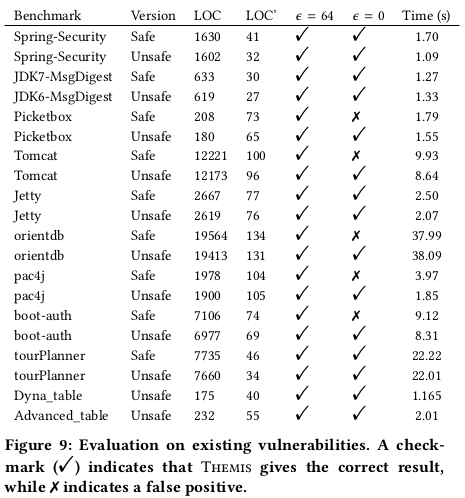
\includegraphics[scale=0.36]{img_chen/9.png}
  \end{center}
 Average: 8.81 seconds.
\end{frame}

\begin{frame}{Zero-Days Vulnerabilities}
  \begin{center}
    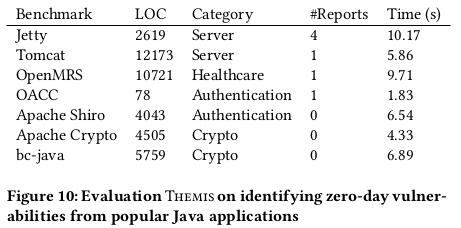
\includegraphics[scale=0.4]{img_chen/10.png}
  \end{center}
  6 out of 7 already fixed. One false alarm.
  \begin{center}
    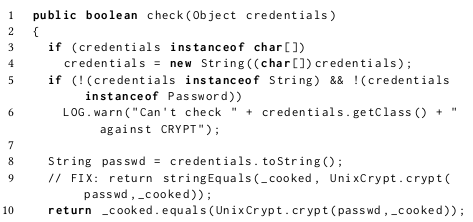
\includegraphics[scale=0.4]{img_chen/11.png}
  \end{center}
\end{frame}

\begin{frame}{Conclusion}
  \begin{alertblock}{Limitations}
  \begin{itemize}
  \item False Alarms.
  \item No Recursive functions.
  \item Some JAVA features are missing.
  \item Only software vulnerabilities.
  \end{itemize}
  \end{alertblock}
  \vfill
  \begin{exampleblock}{Results}
    \begin{itemize}
    \item Better definition of non-interference.
    \item New sound Hoare Logic and verification algorithm.
    \item Implementation of \textsc{Themis}. Compares favorably against \textsc{Blazer}
    \item New bugs found.
    \end{itemize}
  \end{exampleblock}
\end{frame}


\end{document}
